\documentclass{article}
\usepackage[top=5mm]{geometry}
\usepackage{graphicx}
\usepackage{wrapfig}
\graphicspath{ {images/} }
\date{}

\begin{document}

\title{MANAN ANAND}
\maketitle
\vspace{-2cm}

\begin{center}

{\large 269 SATYA NIKETAN\\
NEW DELHI-21\\
9910831722,manananand11@gmail.com\par} 
\end{center}
\noindent\rule{15cm}{1pt}


\begin{wrapfigure}{r}{0.25\textwidth}
    \centering
    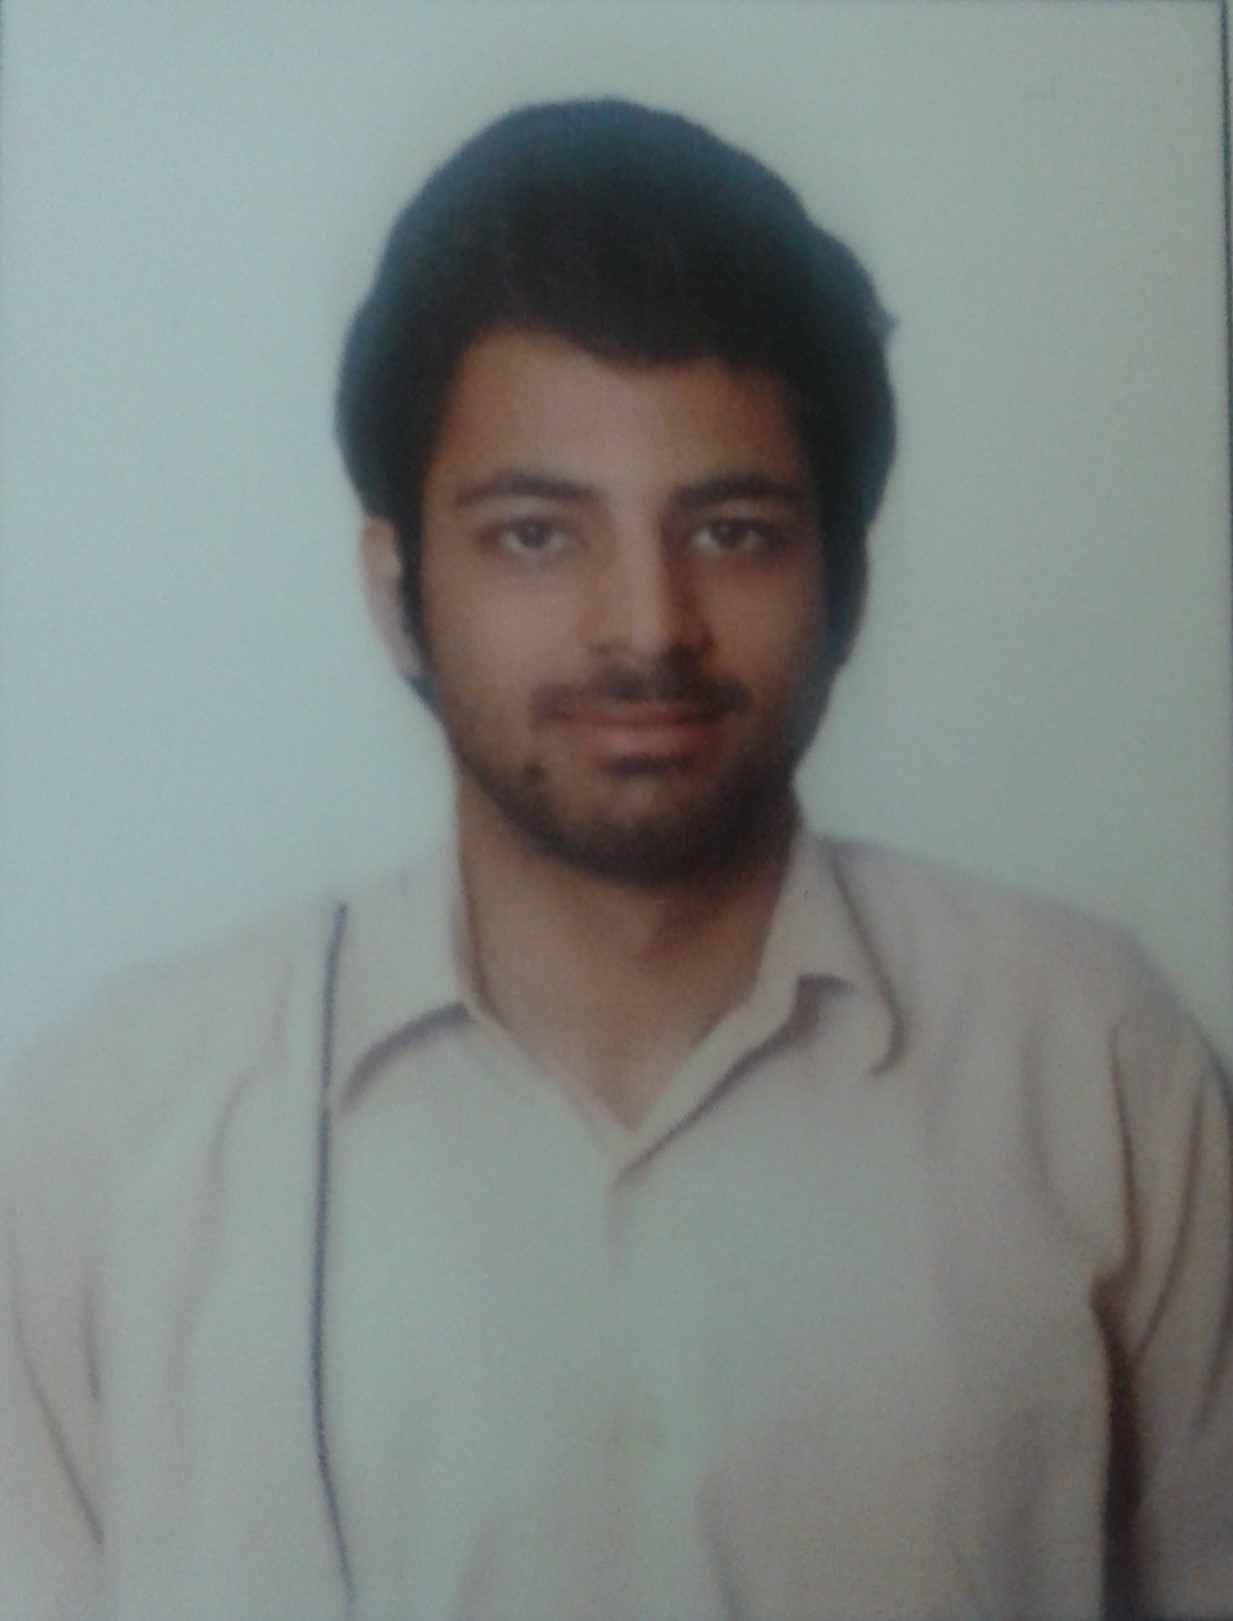
\includegraphics[width=0.25\textwidth]{manan_resume}
\end{wrapfigure}

SIC10,\\
ERTS Lab,\\
IIT Bombay, Powai,\\
Mumbai-400076,\\
Maharashtra

\section{OBJECTIVE EDUCATION}
\begin{center}
 SCHOOL
\end{center}

\begin{tabular}{ |c|c|c| } 
 \hline
 CLASS  & PASSING YEAR & PASS PERCENTAGE \\ 
\hline
 10TH & 2014 & 8.6 C.G.P.A \\ 
 12TH & 2016 & 92.6\% \\ 
 \hline
\end{tabular}

\large Currently Pursuing B.Tech in Electronics And Communication from Bharati Vidyapeeth's College of engineering, New Delhi

\section{PROJECTS}
\Large
\begin{enumerate}
\item Made a game in Blender 3D. 
\item Made a conveyor belt using waste materials.
\item Worked on a Differential Drive using Bluetooth Module.
\end{enumerate}

\section{INTERNSHIP}
Did an Internship at Cache Infotech in 2015.

\section{SKILLS}
\begin{enumerate}
\item 3D Modelling in Blender 3D
\item Mechanical skills
\end{enumerate}

\section{SOFT SKILLS}
1. Communication Skills\\
2. Leadership\\
3. Teamwork\\
4. Time Management\\

\section{EXTRA-CIRRICULAR ACTIVITIES}
\begin{enumerate}
\item Executive Technical Head in Computer Society of India
\item Conducted an event at FELICITY in Bharati Vidyapeeth's College of Engineering
\end{enumerate}

\section{CO-CURRICULAR ACTIVITIES}
\begin{enumerate}
\item Participated In Robo Race at Delhi Technological University and came 5th out of 50 teams.
\item Participated in Robo Push at Bharati Vidyapeeths ISTE Fest and Secured The First Position.
\item Participated in E-Yantra Robotics Competition and Secured the 4th position at the National Finals.
\item Secured First position in best out of waste competition at school level.
\end{enumerate}

\end{document}